%!TEX program=xelatex
\documentclass{article}

% Chinese font
\usepackage{xeCJK}
\usepackage{hyperref}

\setCJKmainfont{[kaiu.ttf]}
\setmainfont{[times new roman.ttf]}

\usepackage{colortbl}
\usepackage{xcolor}

\definecolor{LightGray}{gray}{0.8}
\newcolumntype{a}{>{\columncolor{LightGray}}c}

\usepackage{tabularx}
\usepackage{makecell}

\setcounter{section}{-1}
\renewcommand*\contentsname{目錄}

\usepackage{graphicx}

\graphicspath{{./img/}}

\usepackage{indentfirst}

\begin{document}
\begin{titlepage}
	\centering

	{\huge 海大教室借用平台}

	\vfill

	{\huge 需求規格文件}

	\vfill

	\begin{Large}
		\begin{center}
			\begin{tabular}{| a | c |}
				\hline
				專案名稱 & 海大教室借用平台               \\ \hline
				撰寫日期 & \today                 \\ \hline
				發展者  & \makecell{曾昱翔、林暐傑、陳鈺翔、 \\張銀軒、黃見弘} \\ \hline
			\end{tabular}
		\end{center}
	\end{Large}
\end{titlepage}


\addcontentsline{toc}{section}{版次變更紀錄}
\section*{版次變更紀錄}

\begin{tabularx}{\textwidth}{| c | X | X |}
	\rowcolor{LightGray}
	\hline
	版次    & 變更項目              & 變更日期       \\ \hline
	0.1   & 初版                & 2022/10/04 \\ \hline
	0.1.1 & 加入 User Story Map & 2022/10/13 \\ \hline
	0.1.2 & 完成系統概述            & 2022/10/14 \\ \hline
	0.1.3 & 完成使用者介面分析         & 2022/10/19 \\ \hline
	      &                   &            \\ \hline
	      &                   &            \\ \hline
\end{tabularx}

\newpage

\begin{center}
	\tableofcontents
\end{center}

\newpage

\section[接受準則(ACCEPTANCE CRITERIA OF THIS DOCUMENT)]{接受準則(Accpetance Criteria of this Document)}


\begin{itemize}
	\color{blue}
	\item Clearly and properly stated (需求需清楚且適當的陳述)
	\item Complete (需求需完整)
	\item Consistent with each other (需求之間需維持一致性)
	\item Uniquely identified (每項需求有明確之識別)
	\item Appropriate to implement (需求需可被實作)
	\item Verifiable (需求需可被驗證)
\end{itemize}

\newpage

\section[系統概述(SYSTEM DESCRIPTION)]{系統概述(System Description)}

隨著各種服務數位化,許多事情能夠在網路上處理就不需要到現場,例如網路銀行、網路購物、網路訂票等等,這些服務都能夠讓人們在家中就能夠完成,節省了許多時間,也讓人們的生活更加便利。
然而,許多學校的教室借用系統仍然是以紙本的方式來處理,這樣的方式不僅浪費了許多紙張,也讓人們在借用教室時需要花費許多時間,因此我們希望能夠開發一個網路教室借用系統,讓人們能夠在網路上借用教室,並且能夠在借用教室時節省許多時間。

\subsection{系統目標}

透過網路平台的方式,讓使用者可以在任何地方,隨時隨地的借用教室,並即時的得知教室借用的狀態。

\subsection{系統特色}

使用人性化的介面和即時的狀態顯示,整合 Email 通知系統,除了讓使用者能避免到現場登記借用教室外,也能在借用教室時節省許多時間。

\bigskip

對於管理者而言,透過數位的紀錄方式,能夠更有效的管理教室借用的紀錄等資訊,更直觀的分配教室,並且能夠即時的得知教室借用的狀態。

\newpage

\section[使用者故事地圖(USER STORY MAP)]{使用者故事地圖(User Story Map)}

\begin{center}
	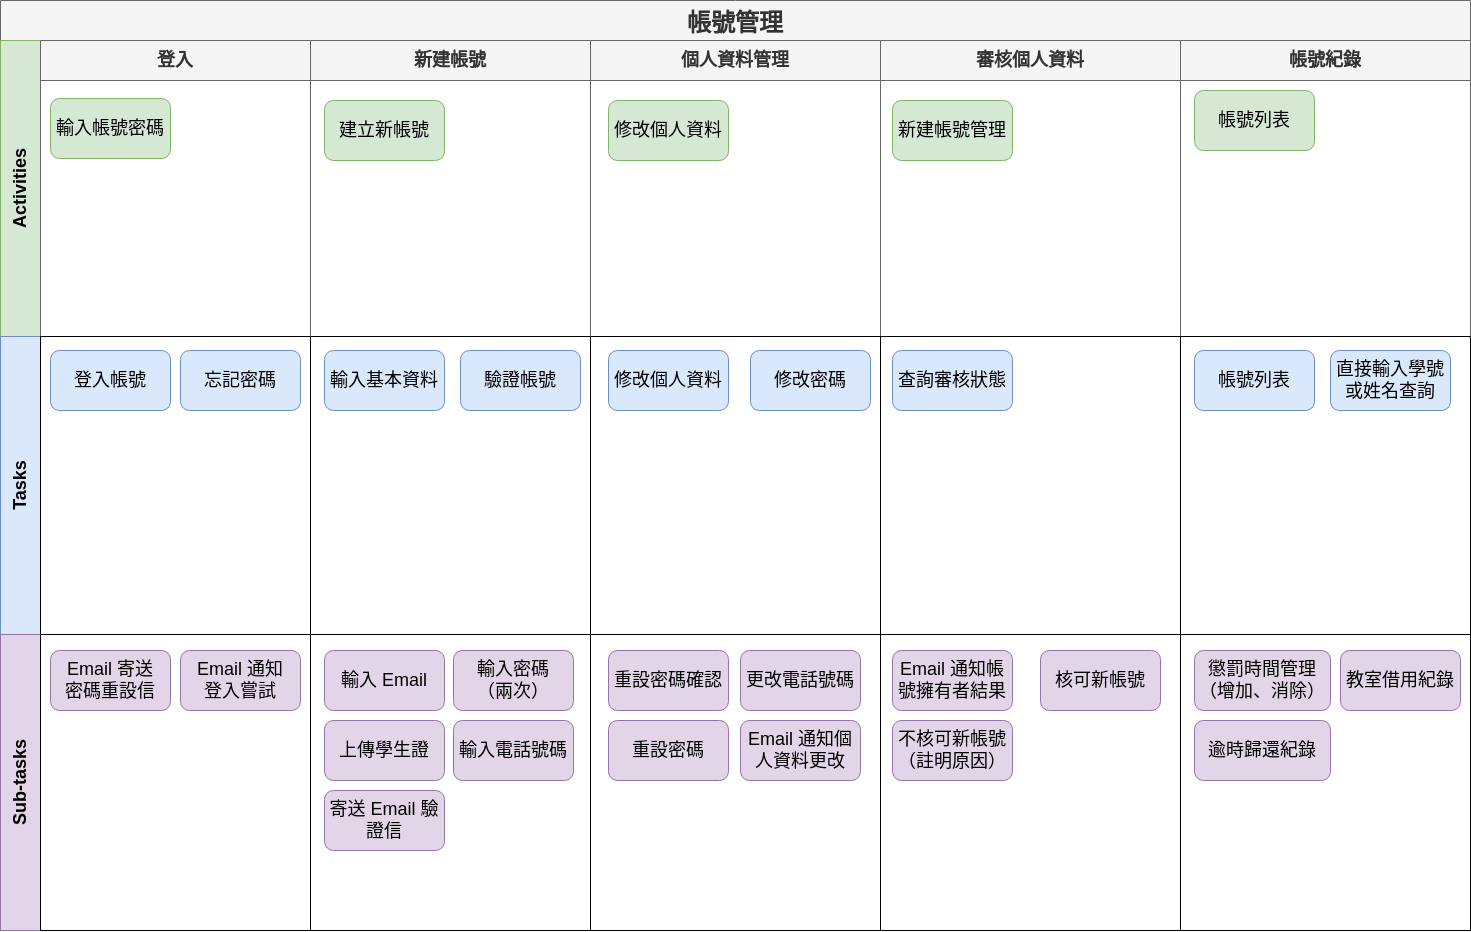
\includegraphics[height=0.45\textheight]{UserStoryMap-AccountManagement.png}
\end{center}

\begin{center}
	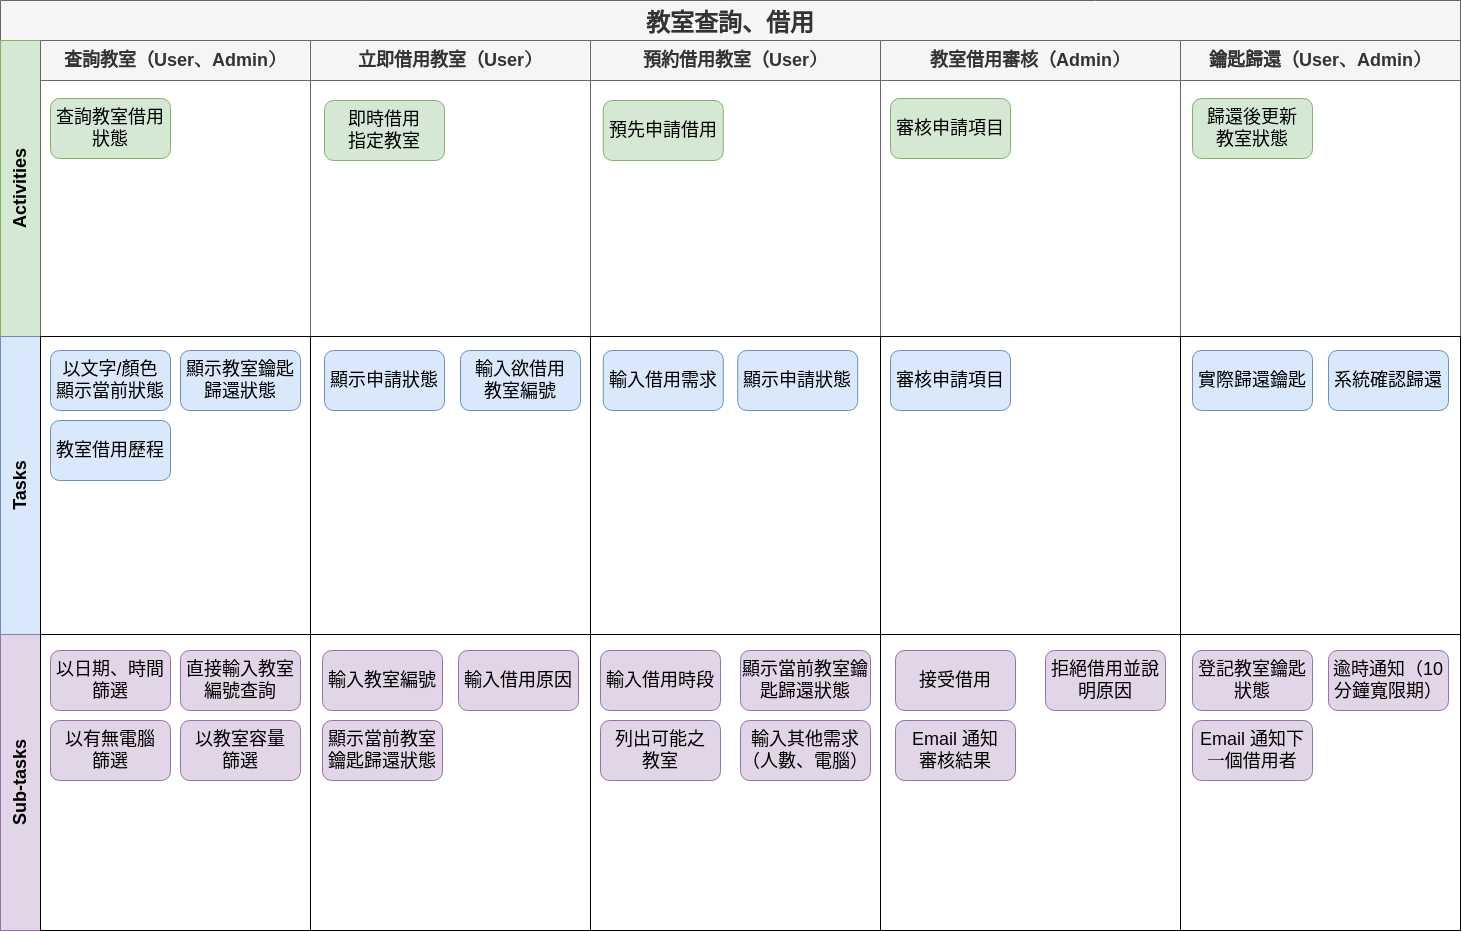
\includegraphics[height=0.45\textheight]{UserStoryMap-ClassroomBorrowing.png}
\end{center}

\newpage

\section[操作概念(OPERATIONAL CONCEPTS)]{操作概念(Operational Concepts)}

\newpage

\section[功能需求(FUNCTIONAL REQUIREMENTS)]{功能需求(Functional Requirements)}
\begin{tabular}{|l|c|c|}
	\hline
	功能編號                      & 功能名稱   & 功能說明                        \\ \hline
	\multicolumn{3}{| c |}{Account Management(帳號管理)}                 \\ \hline
	CBP-AM-LOG-01             & 帳號登入   & 使用者/管理員可於登入介面登入帳號           \\ \hline
	CBP-AM-REG-01             & 帳號註冊   & 使用者可使用 Email 與自訂密碼進行註冊      \\ \hline
	CBP-AM-PIM-01             & 個人資料管理 & 使用者可更改密碼與電話號碼               \\ \hline
	\color{blue}CBP-AM-PIV-01 & 審核個人資料 & 管理員可根據 Email 認證結果核可/否決新辦帳號  \\ \hline
	\color{blue}CBP-AM-AR-01  & 帳號紀錄   & 管理員可根據學號/姓名等資訊查詢使用者使用紀錄     \\ \hline
	\multicolumn{3}{| c |}{Classroom Borrowing \& Inquiring(教室租借查詢)} \\ \hline
	CBP-CBI-LOG-01            & 教室查詢   & 使用者可查詢教室目前使用狀態              \\ \hline
	CBP-CBI-BOR-01            & 教室立即借用 & 使用者可輸入教室編號進行借用              \\ \hline
	CBP-CBI-BOR-02            & 教室預約借用 & 使用者可輸入時段及需求進行申請             \\ \hline
	\color{blue}CBP-CBI-BOR-3 & 預約審核   & 管理員可對預約進行審核                 \\ \hline
	\color{blue}CBP-CBI-KR-1  & 鑰匙歸還登記 & 管理員可變更教室狀態                  \\ \hline
\end{tabular}
\newpage

\section[非功能需求(NON-FUNCTIONAL REQUIREMENTS)]{非功能需求(Non-Functional Requirements)}

\newpage

\section[使用者介面分析(USER INTERFACE ANALYSIS)]{使用者介面分析(User Interface Analysis)}

\begin{minipage}{0.6\linewidth}
	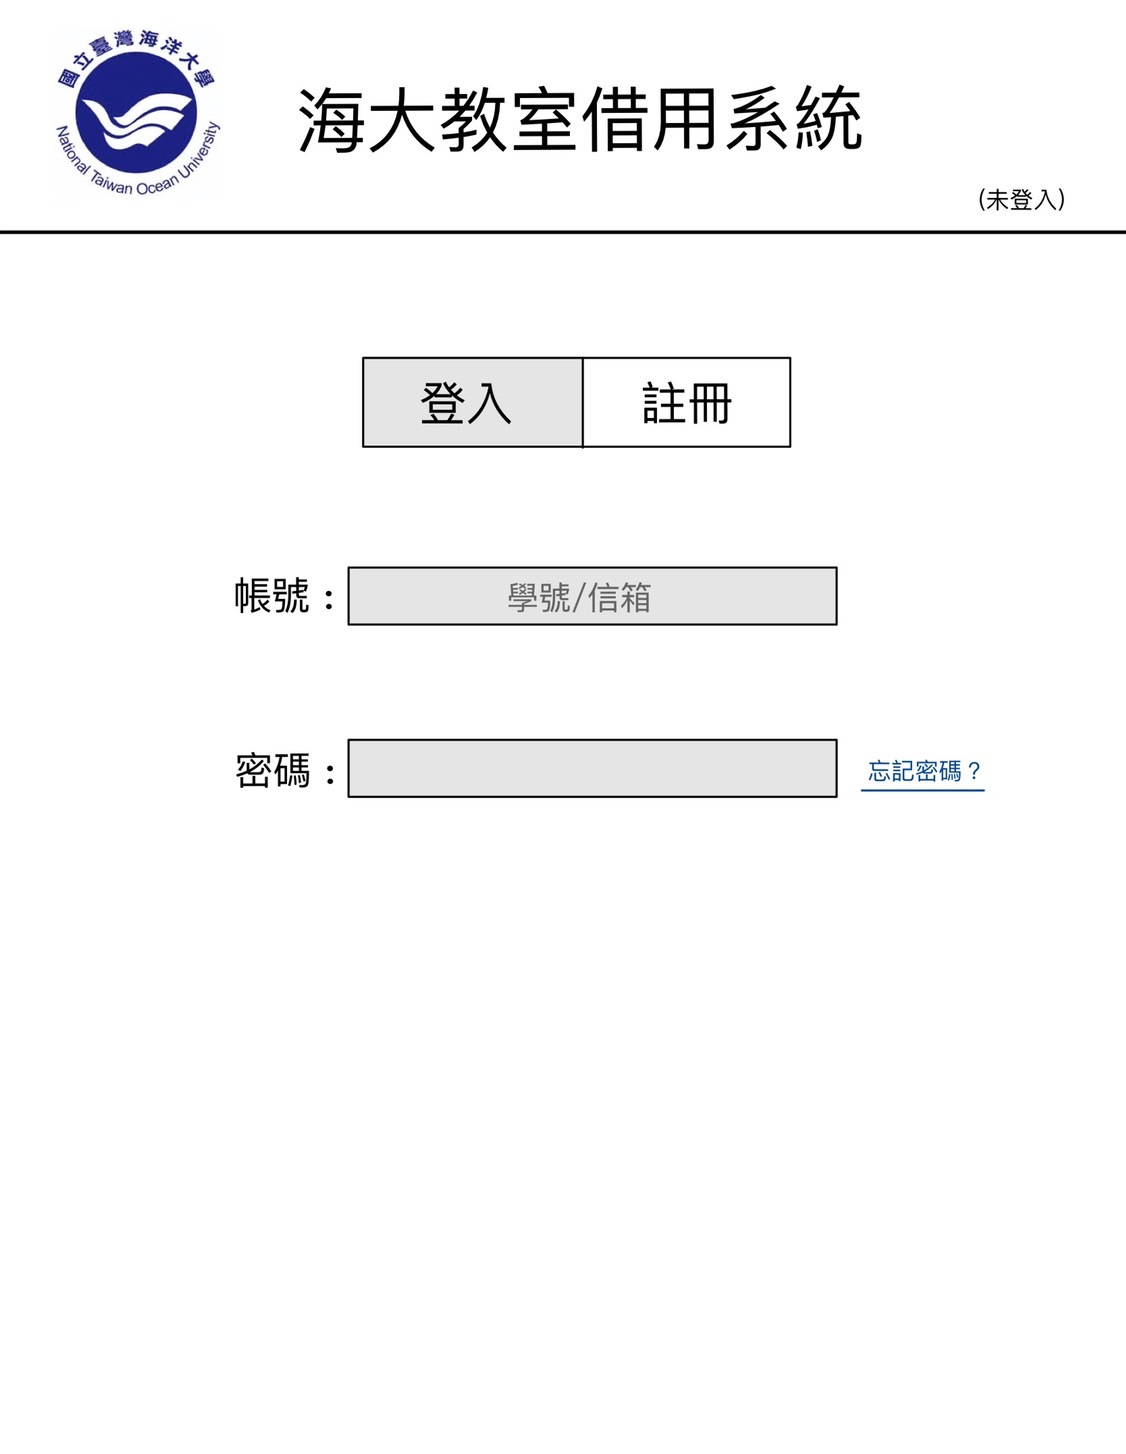
\includegraphics[height=0.4\textheight]{Log_In_GUI.jpg}
\end{minipage}
\begin{minipage}{0.4\linewidth}
	\subsection*{登入介面:}使用者可輸入學號/Email及密碼進行登入、或使用忘記密碼功能
\end{minipage}

\begin{minipage}{0.6\linewidth}
	\subsection*{註冊介面:}使用者可輸入學號、Email帳號並重複兩次自訂密碼註冊
\end{minipage}
\begin{minipage}{0.4\linewidth}
	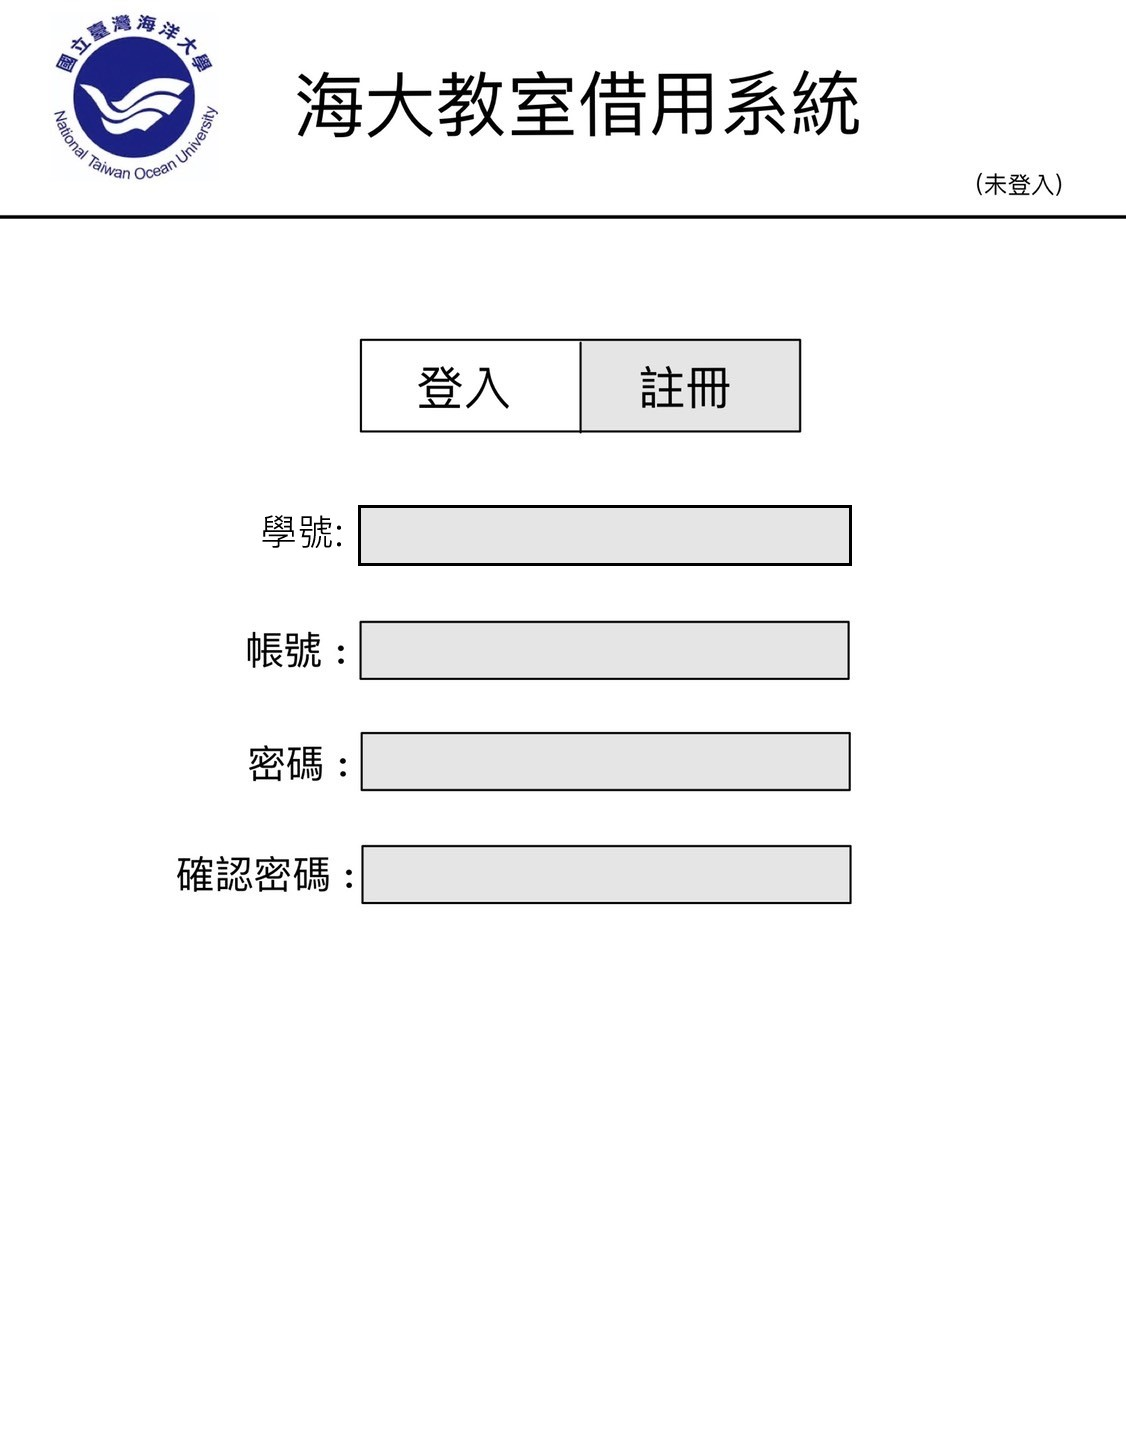
\includegraphics[height=0.4\textheight]{Regester_GUI.jpg}
\end{minipage}

\newpage
\subsection*{教室借用介面:}
\medskip
\begin{minipage}{0.6\linewidth}
	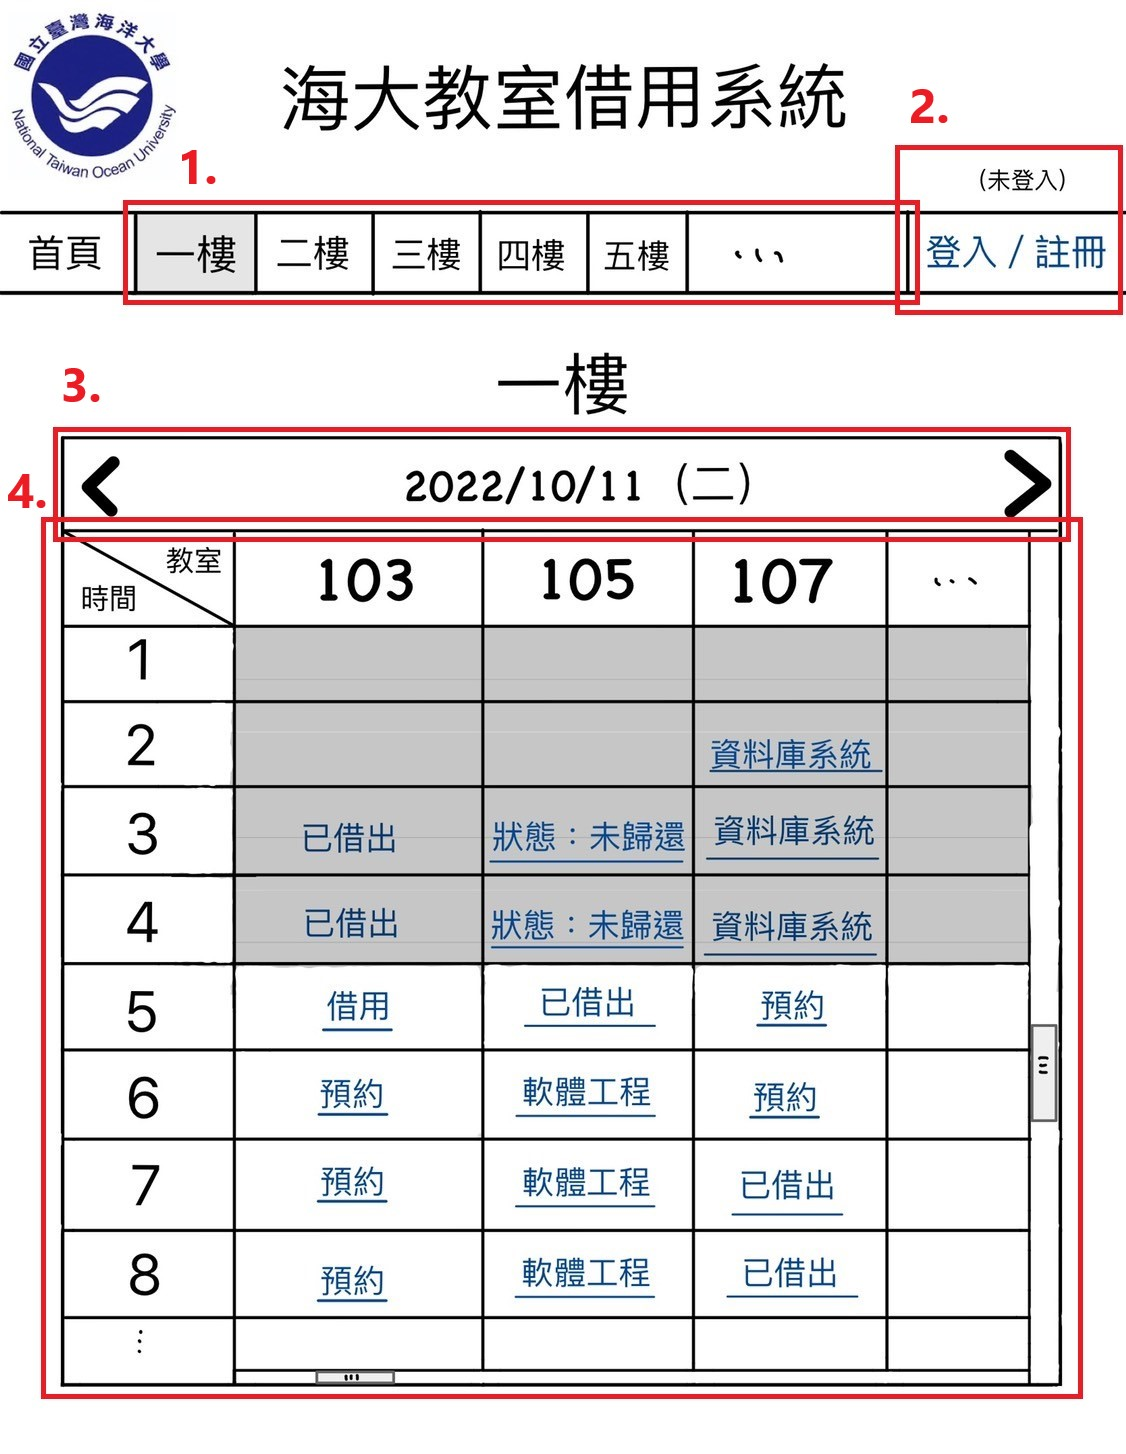
\includegraphics[height=0.4\textheight]{Borowing_GUI.jpg}
\end{minipage}
\begin{minipage}{0.4\linewidth}
	\subsubsection*{\textcolor{red}{1.}樓層選擇:}可選擇系館樓層
	\subsubsection*{\textcolor{red}{2.}登入狀態:}可按此登入、登出
	\subsubsection*{\textcolor{red}{3.}日期選擇:}可選擇欲借用之日期
	\subsubsection*{\textcolor{red}{4.}教室狀態:}直行為時間、橫列為教室,教室狀態有:已有固定課程、已經借用、尚未歸還鑰匙、可借用
\end{minipage}

\end{document}
